\appendix
% \renewcommand{\appendixname}{附录~\Alph{section}}
% \renewcommand{\appendixtocname}{附录}
% \addappheadtotoc
% \renewcommand{\appendixpagename}{\centering 附录}
% \appendixpage

% \begin{appendices}

% \heiti
% \zihao{3}

\section*{附\ \ \ \ 录\ \ \ }

\addcontentsline{toc}{section}{附\ \ \ \ 录}

\renewcommand{\thesubsection}{附录\Alph{subsection}}
% \renewcommand\thetable{\thesection.\arabic{table}}
% \renewcommand\thefigure{\arabic{figure}}

\newcommand{\appendsection}[1]{\titleformat*{\subsection}{\centering}\zihao{-4}\heiti\subsection{} {\centering\paragraph{#1}\mbox{}\\}\songti}
\newcommand{\appendchn}[1]{\titleformat*{\subsection}{\centering}\zihao{-4}\heiti\subsection*{中文译文\Alph{subsection}} {\centering\paragraph{#1}\mbox{}\\}\songti}

% \renewcommand{\figurename}{图 A.}
% \setcounter{figure}{0}

% \titlespacing*{\subsection}{-20pt}{*1.5}{*1.1}


\appendsection{Raft - In Search of an Understandable Consensus Algorithm}

Raft is a consensus algorithm for managing a replicated log. It provides the same function and performance as the Paxos algorithm, but its algorithm structure is different from Paxos, making the Raft algorithm easier to understand and easier to build an actual system. To improve understandability, Raft decomposes the consensus algorithm into several key modules, such as leader election, log replication, and security. At the same time it reduces the number of states that need to be considered by enforcing a stronger consistency. The results of a user study show that the Raft algorithm is easier for students to learn than the Paxos algorithm. The Raft algorithm also includes a new mechanism to allow dynamic changes in cluster membership, which utilizes overlapping majorities for safety.
Consensus algorithms allow a group of machines to work as a whole and continue to work even if some of them fail. Because of this, consensus algorithms play an important role in building trustworthy large-scale software systems. For the past 10 years, the Paxos algorithm has dominated the field of consensus algorithms: the vast majority of implementations are based on or influenced by Paxos. At the same time, Paxos has also become an example in the teaching field when explaining consistency issues.

But unfortunately, the Paxos algorithm is still very difficult to understand despite a lot of work trying to reduce its complexity. Moreover, the algorithm structure of Paxos itself needs to be greatly modified before it can be applied to the actual system. Therefore, both industry and academia are very troubled by the Paxos algorithm.
After working hard on the Paxos algorithm, we set out to find a new consensus algorithm that could provide a better basis for building practical systems and teaching. Unlike Paxos, our primary goal is understandability: can we define a consensus algorithm in real systems that is easier to learn than the Paxos algorithm. Furthermore, we hope that the algorithm facilitates the development of the system builder's intuition. It's not just that the algorithm works, it's that you know exactly why it works.
The Raft consensus algorithm is the result of this work. When designing the Raft algorithm, we use some special techniques to improve its understandability, including algorithm decomposition (Raft is mainly divided into three modules of leader election, log replication and security) and reducing the state of the state machine (compared to Like Paxos, Raft reduces non-determinism and the way servers are inconsistent with each other). A study of 43 students at two universities showed that Raft is significantly easier to understand than Paxos. After these students learned both algorithms, 33 of them were able to answer questions about Raft compared to Paxos.

Consensus algorithms are proposed in the context of replicated state machines. In this approach, a state machine on a set of servers produces a copy of the same state and can continue to run even if some machines go down. Replicated state machines are used in distributed systems to solve many fault tolerance problems. For example, there is usually a cluster leader in large-scale systems, such as GFS, HDFS and RAMCloud, and a typical application is an independent replication state machine to manage leader election and store configuration information survived. Such as Chubby and ZooKeeper.
A consensus algorithm manages a replicated log of instructions from clients. The state machine processes the same instructions in the same order from the log, so the results are the same.

Replicated state machines are usually implemented based on replicated logs. Each server stores a log containing a series of instructions and executes them in the order of the log. Every log contains the same commands in the same order, so every server executes the same sequence of commands. Because every state machine is deterministic, every execution of an operation produces the same state and the same sequence.

The task of the consensus algorithm is to ensure the consistency of the replicated log. The consistency module on the server receives the instructions sent by the client and adds them to its own log. It communicates with consistency modules on other servers to ensure that the logs on each server eventually contain the same requests in the same order, even if some servers fail. Once the commands are replicated correctly, each server's state machine processes them in log order, and the output is returned to the client. Thus, the cluster of servers appears to form a highly reliable state machine.

Consensus algorithms used in practical systems usually have the following characteristics:
Safety guarantee (never return a wrong result): In the case of non-Byzantine errors, errors including network delays, partitions, packet loss, duplication, and disorder are guaranteed to be correct.
Availability: As long as most of the machines in the cluster are operational and able to communicate with each other and clients, they can be guaranteed to be available. Therefore, a typical cluster of 5 nodes can tolerate the failure of two nodes. A server is considered a failure if it is stopped. They may later recover from the reliably stored state and rejoin the cluster.
Do not rely on timing for consistency: physical clock errors or extreme message delays cause availability problems only in the worst case.
Typically, an instruction can complete as quickly as possible when most nodes in the cluster respond to a round of remote procedure calls. A small number of slower nodes will not affect the overall performance of the system.





% \begin{titlepage}
% 	\includepdf[fitpaper]{other/Raft}
% \end{titlepage}

\appendchn{Raft-一种易于理解的共识性算法}

Raft 是一种为了管理复制日志的一致性算法。它提供了和 Paxos 算法相同的功能和性能,但是它的算法结构和 Paxos 不同,使得 Raft 算法更加容易理解并且更容易构建实际的系统。为了提升可理解性,Raft 将一致性算法分解成了几个关键模块,例如领导人选举、日志复制和安全性。同时它通过实施一个更强的一致性来减少需要考虑的状态的数量。一项用户研究的结果表明,对于学生而言,Raft 算法比 Paxos 算法更加容易学习。Raft 算法还包括一个新的机制来允许集群成员的动态改变,它利用重叠的大多数来保证安全性。
一致性算法允许一组机器像一个整体一样工作,即使其中一些机器出现故障也能够继续工作下去。正因为如此,一致性算法在构建可信赖的大规模软件系统中扮演着重要的角色。在过去的 10 年里,Paxos 算法统治着一致性算法这一领域:绝大多数的实现都是基于 Paxos 或者受其影响。同时 Paxos 也成为了教学领域里讲解一致性问题时的示例。

但是不幸的是,尽管有很多工作都在尝试降低它的复杂性,但是 Paxos 算法依然十分难以理解。并且,Paxos 自身的算法结构需要进行大幅的修改才能够应用到实际的系统中。因此工业界和学术界都对 Paxos 算法感到十分头疼。
努力研究过 Paxos 算法之后,本文开始寻找一种新的一致性算法,可以为构建实际的系统和教学提供更好的基础。与 Paxos 不同,本文的首要目标是可理解性:本文是否可以在实际系统中定义一个一致性算法,并且比 Paxos 算法更容易学习。此外,本文希望该算法方便系统构建者的直觉的发展。重要的不仅仅是算法能够工作,更重要的是能够很清楚地知道它为什么能工作。
Raft 一致性算法就是这些工作的结果。在设计 Raft 算法的时候,本文使用一些特别的技巧来提升它的可理解性,包括算法分解(Raft 主要被分成了领导人选举,日志复制和安全三个模块)和减少状态机的状态(相对于 Paxos,Raft 减少了非确定性和服务器互相处于非一致性的方式)。一份针对两所大学 43 个学生的研究表明 Raft 明显比 Paxos 算法更加容易理解。在这些学生同时学习了这两种算法之后,和 Paxos 比起来,其中 33 个学生能够回答有关于 Raft 的问题。

一致性算法是从复制状态机的背景下提出的。在这种方法中,一组服务器上的状态机产生相同状态的副本,并且在一些机器宕掉的情况下也可以继续运行。复制状态机在分布式系统中被用于解决很多容错的问题。例如,大规模的系统中通常都有一个集群领导人,像 GFS、HDFS 和 RAMCloud,典型应用就是一个独立的复制状态机去管理领导选举和存储配置信息并且在领导人宕机的情况下也要存活下来。比如 Chubby 和 ZooKeeper。
一致性算法管理着来自客户端指令的复制日志。状态机从日志中处理相同顺序的相同指令,所以产生的结果也是相同的。

复制状态机通常都是基于复制日志实现的。每一个服务器存储一个包含一系列指令的日志,并且按照日志的顺序进行执行。每一个日志都按照相同的顺序包含相同的指令,所以每一个服务器都执行相同的指令序列。因为每个状态机都是确定的,每一次执行操作都产生相同的状态和同样的序列。

一致性算法的任务是保证复制日志的一致性。服务器上的一致性模块接收客户端发送的指令然后添加到自己的日志中。它和其它服务器上的一致性模块进行通信来保证每一个服务器上的日志最终都以相同的顺序包含相同的请求,即使有些服务器发生故障。一旦指令被正确的复制,每一个服务器的状态机按照日志顺序处理它们,然后输出结果被返回给客户端。因此,服务器集群看起来形成了一个高可靠的状态机。

实际系统中使用的一致性算法通常含有以下特性:
安全性保证(绝对不会返回一个错误的结果):在非拜占庭错误情况下,包括网络延迟、分区、丢包、重复和乱序等错误都可以保证正确。
可用性:集群中只要有大多数的机器可运行并且能够相互通信、和客户端通信,就可以保证可用。因此,一个典型的包含 5 个节点的集群可以容忍两个节点的失败。服务器被停止就认为是失败。它们稍后可能会从可靠存储的状态中恢复并重新加入集群。
不依赖时序来保证一致性:物理时钟错误或者极端的消息延迟只有在最坏情况下才会导致可用性问题。
通常情况下,一条指令可以尽可能快的在集群中大多数节点响应一轮远程过程调用时完成。小部分比较慢的节点不会影响系统整体的性能。





\appendsection{The Log-Structured Merge-Tree}


High-performance transaction system applications typically insert rows in a
History table to provide an activity trace; at the same time the transaction system generates log
records for purposes of system recovery. Both types of generated information can benefit from
efficient indexing. An example in a well-known setting is the TPC-A benchmark application,
modified to support efficient queries on the History for account activity for specific accounts.
This requires an index by account-id on the fast-growing History table. Unfortunately, stan-
dard disk-based index structures such as the B-tree will effectively double the I/O cost of the
transaction to maintain an index such as this in real time, increasing the total system cost up to
fifty percent. Clearly a method for maintaining a real-time index at low cost is desirable. The
Log-Structured Merge-tree (LSM-tree) is a disk-based data structure designed to provide
low-cost indexing for a file experiencing a high rate of record inserts (and deletes) over an
extended period. The LSM-tree uses an algorithm that defers and batches index changes, cas-
cading the changes from a memory-based component through one or more disk components in an
efficient manner reminiscent of merge sort. During this process all index values are contin-
uously accessible to retrievals (aside from very short locking periods), either through the
memory component or one of the disk components. The algorithm has greatly reduced disk arm
movements compared to a traditional access methods such as B-trees, and will improve cost-
performance in domains where disk arm costs for inserts with traditional access methods
overwhelm storage media costs. The LSM-tree approach also generalizes to operations other
than insert and delete. However, indexed finds requiring immediate response will lose I/O ef-
ficiency in some cases, so the LSM-tree is most useful in applications where index inserts are
more common than finds that retrieve the entries. This seems to be a common property for
History tables and log files, for example. The conclusions of Section 6 compare the hybrid use
of memory and disk components in the LSM-tree access method with the commonly understood
advantage of the hybrid method to buffer disk pages in memory.

As long-lived transactions in activity flow management systems become commercially available
 there will be increased need to provide indexed access
to transactional log records. Traditionally, transactional logging has focused on aborts and re-
covery, and has required the system to refer back to a relatively short-term history in normal
processing with occasional transaction rollback, while recovery was performed using batched
sequential reads. However, as systems take on responsibility for more complex activities, the
duration and number of events that make up a single long-lived activity will increase to a point
where there is sometimes a need to review past transactional steps in real time to remind users
of what has been accomplished. At the same time, the total number of active events known to a
system will increase to the point where memory-resident data structures now used to keep
track of active logs are no longer feasible, notwithstanding the continuing decrease in memory
cost to be expected. The need to answer queries about a vast number of past activity logs implies
that indexed log access will become more and more important.

Even with current transactional systems there is clear value in providing indexing to support
queries on history tables with high insert volume. Networking, electronic mail, and other
nearly-transactional systems produce huge logs often to the detriment of their host systems. To
start from a concrete and well-known example, we explore a modified TPC-A benchmark in the
following Examples 1.1 and 1.2. Note that examples presented in this paper deal with specific
numeric parametric values for ease of presentation; it is a simple task to generalize these
results. Note too that although both history tables and logs involve time-series data, the index
entries of the LSM-Tree are not assumed to have indentical temporal key order. The only as-
sumption for improved efficiency is high update rates compared to retrieval rates.

% \begin{titlepage}
% 	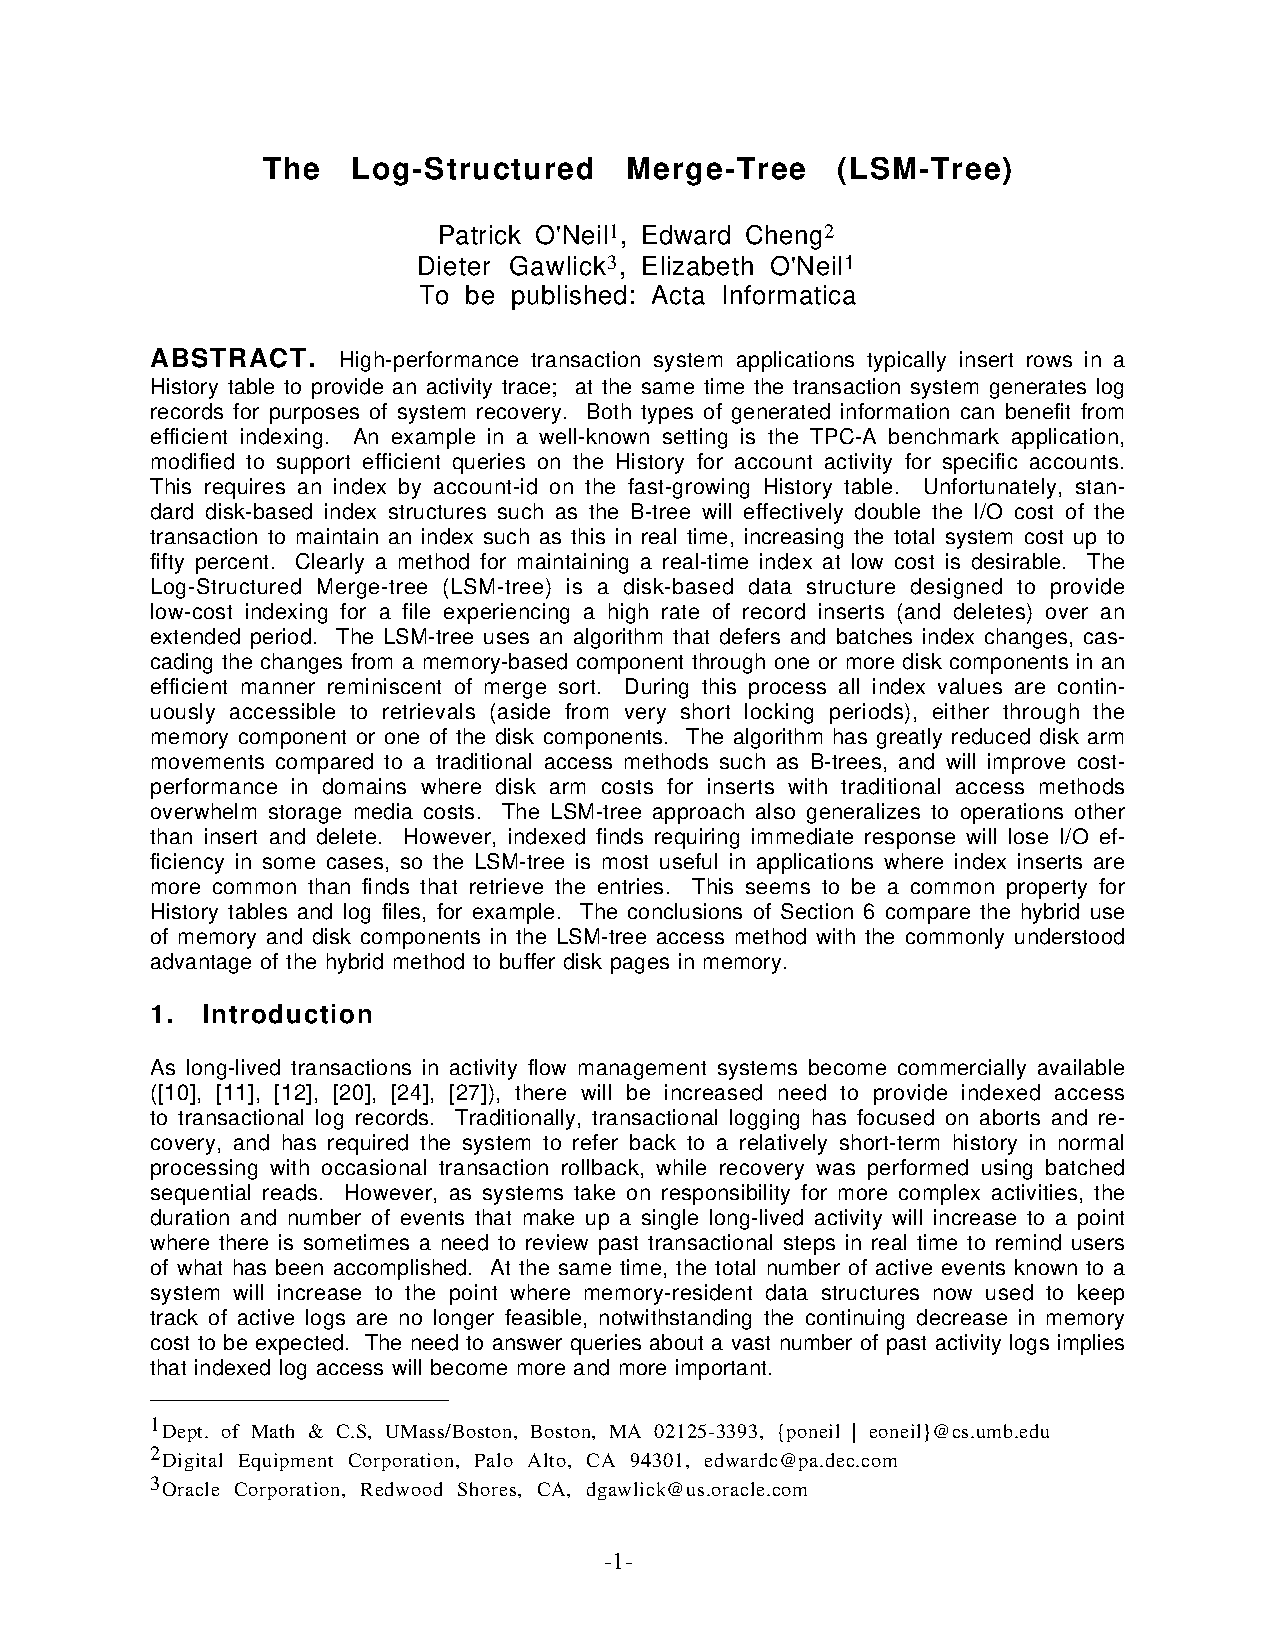
\includepdf[fitpaper]{other/lsmtree}
% \end{titlepage}

\appendchn{日志结构归并树}


高性能事务系统应用程序通常在一个
提供活动轨迹的历史表; 同时交易系统产生日志
用于系统恢复的记录。 两种类型的生成信息都可以从中受益
高效的索引。 一个众所周知的例子是 TPC-A 基准应用程序,
修改以支持对特定帐户的帐户活动历史记录进行有效查询。
这需要在快速增长的 History 表上按 account-id 建立索引。 不幸的是,斯坦-
基于硬磁盘的索引结构,如 B-tree 将有效地使 I/O 成本加倍
事务来实时维护这样的索引,增加了总系统成本高达
百分之五十。 显然,需要一种以低成本维护实时索引的方法。 这
Log-Structured Merge-tree (LSM-tree) 是一种基于磁盘的数据结构,旨在提供
对经历高记录插入(和删除)率的文件进行低成本索引
延展期。 LSM-tree 使用延迟和批处理索引更改的算法,cas-
将来自基于内存的组件的更改缓存到一个或多个磁盘组件中
高效的方式让人联想到归并排序。 在此过程中,所有指标值都在连续
非常容易检索(除了非常短的锁定期),要么通过
内存组件或磁盘组件之一。 该算法大大减少了磁盘臂
与传统的访问方法(如 B 树)相比,移动将提高成本
在使用传统访问方法插入磁盘臂成本的域中的性能
不堪重负的存储介质成本。 LSM-tree 方法也推广到其它操作
比插入和删除。 然而,需要立即响应的索引查找将丢失 I/O ef-
在某些情况下效率很高,因此 LSM-tree 在需要插入索引的应用程序中最有用
比检索条目的发现更常见。 

随着活动流管理系统中的长期交易变得商业可用
  提供索引访问的需求将增加
到事务日志记录。 传统上,事务日志集中于中止和重新
覆盖,并要求系统在正常情况下返回相对较短的历史记录
处理偶尔的事务回滚,而恢复是使用批处理执行的
顺序读取。 然而,随着系统承担起更复杂活动的责任,
构成单个长期活动的持续时间和事件数量将增加到一个点
有时需要实时回顾过去的交易步骤以提醒用户
已经完成的事情。 同时,已知的活动事件总数
系统将增加到内存驻留数据结构现在用于保存的程度
尽管内存持续减少,但活动日志的跟踪不再可行
预期的成本。 需要回答有关大量过去活动日志的查询意味着
索引日志访问将变得越来越重要。

即使对于当前的事务系统,提供索引以支持也具有明显的价值
查询具有高插入量的历史表。 网络、电子邮件和其它
近事务性系统会产生大量日志,而这些日志通常会损害其主机系统。 到
从一个具体和众所周知的例子开始,本文探索了一个修改后的 TPC-A 基准。

% \end{appendices}